\documentclass[11pt,a4paper]{article}
\usepackage[utf8]{inputenc}
\usepackage{amsmath,amssymb,amsthm}
\usepackage{xcolor}
\usepackage{geometry}
\usepackage{hyperref}
\usepackage{booktabs}
\usepackage{microtype}
\usepackage{cite}
\usepackage{float}
\usepackage{tabularx}
\usepackage{tikz}
\usetikzlibrary{shapes.geometric,arrows.meta,positioning}

\geometry{margin=1in}

\hypersetup{
    colorlinks=true,
    linkcolor=blue!70!black,
    citecolor=green!50!black,
    urlcolor=blue!80!black
}

\theoremstyle{plain}
\newtheorem{theorem}{Theorem}[section]
\newtheorem{lemma}[theorem]{Lemma}
\newtheorem{proposition}[theorem]{Proposition}
\newtheorem{corollary}[theorem]{Corollary}

\theoremstyle{definition}
\newtheorem{definition}[theorem]{Definition}
\newtheorem{example}[theorem]{Example}

\theoremstyle{remark}
\newtheorem{remark}[theorem]{Remark}

\newcommand{\Q}{\mathbb{Q}}
\newcommand{\Z}{\mathbb{Z}}
\newcommand{\C}{\mathbb{C}}
\newcommand{\F}{\mathbb{F}}
\newcommand{\GL}{\mathrm{GL}}
\newcommand{\SL}{\mathrm{SL}}
\newcommand{\Gal}{\mathrm{Gal}}

\title{\textbf{On the Modularity of Semistable Elliptic Curves\\and the Proof of Fermat's Last Theorem}}
\author{\textbf{Expository Note}}
\date{\today}

\begin{document}

\maketitle

\begin{abstract}
We present a self-contained, rigorous exposition of the proof of Fermat's Last Theorem, synthesized through the modern geometric framework established by Gerhard Frey, Jean-Pierre Serre, Ken Ribet, and Sir Andrew Wiles (with Richard Taylor). Beginning with the classical reduction to prime exponents $p \ge 5$, we construct the Frey elliptic curve associated with a hypothetical non-trivial solution to Fermat's equation. We detail the computation of its minimal discriminant, conductor, and the semistable reduction properties at all primes. By analyzing the associated Galois representation on the $p$-torsion subgroup via Mazur's theorem on rational torsion, we apply Ribet's level-lowering theorem (the Serre $\varepsilon$-conjecture) in conjunction with Wiles' Modularity Theorem for semistable elliptic curves. We demonstrate that this necessitates the existence of a non-trivial cusp form of weight $2$ and level $2$ on $\Gamma_0(2)$. Since the space $S_2(\Gamma_0(2))$ is of dimension zero, an irresolvable contradiction is reached, definitively establishing the theorem.
\end{abstract}

\tableofcontents

\vspace{1em}
\hrule
\vspace{1.5em}

\section{Introduction and Historical Framework}

In 1637, Pierre de Fermat recorded his famous marginal note in Bachet's translation of Diophantus' \emph{Arithmetica}:
\begin{quote}
\emph{``Cubum autem in duos cubos, aut quadratoquadratum in duos quadratoquadratos, et generaliter nullam in infinitum ultra quadratum potestatem in duos eiusdem nominis fas est dividere cuius rei demonstrationem mirabilem sane detexi. Hanc marginis exiguitas non caperet.''}
\end{quote}
In modern notation, this asserts:

\begin{theorem}[Fermat's Last Theorem]
\label{thm:flt}
For any integer $n \ge 3$, the Diophantine equation
\begin{equation}
\label{eq:fermat}
a^n + b^n = c^n
\end{equation}
has no non-trivial integer solutions with $abc \neq 0$.
\end{theorem}

For over three and a half centuries, this conjecture resisted all direct elementary attempts. While Fermat proved the case $n = 4$ using his method of infinite descent, and Leonhard Euler, Adrien-Marie Legendre, and Peter Gustav Lejeune Dirichlet established cases for $n = 3$ and $n = 5$, Ernst Kummer's landmark 19th-century work revealed that unique factorization fails in cyclotomic fields $\Q(\zeta_p)$, introducing ideal numbers and class groups to settle the theorem for all \emph{regular primes}.

The modern resolution, completed in 1994--1995 by Andrew Wiles~\cite{wiles1995} with assistance from Richard Taylor~\cite{taylorwiles1995}, bypassed direct cyclotomic factorization entirely. Instead, it connected Fermat's equation to the deep interplay between algebraic geometry and complex analysis known as the \emph{Langlands Program}, specifically the \emph{Modularity Theorem} for elliptic curves~\cite{ddt1997, diamondshurman2005}. Recently, this proof was also completely machine-verified in the Lean 4 proof assistant~\cite{anthropic2026, prove2me2026}.

\section{Classical Reductions}

To establish Theorem~\ref{thm:flt} for all $n \ge 3$, elementary reductions suffice to restrict the problem to odd primes:

\begin{lemma}[Reduction to Prime Exponents]
To prove Theorem~\ref{thm:flt}, it is necessary and sufficient to prove:
\begin{enumerate}
    \item Equation~\eqref{eq:fermat} has no non-trivial solutions for $n = 4$.
    \item Equation~\eqref{eq:fermat} has no non-trivial solutions for any odd prime $p \ge 3$.
\end{enumerate}
\end{lemma}
\begin{proof}
Any integer $n \ge 3$ either has an odd prime factor $p$ (so $n = p \cdot k$) or is a power of 2 with $n = 4 \cdot k$. If $(a, b, c)$ satisfies $a^{m k} + b^{m k} = c^{m k}$, then $(a^k, b^k, c^k)$ satisfies $x^m + y^m = z^m$. Hence, non-existence for prime exponents and $n = 4$ precludes solutions for all composite powers.
\end{proof}

The case $n = 4$ was resolved by Fermat via the parameterization of Pythagorean triples and descent on the area of right triangles. The case $p = 3$ was resolved by Euler. We thus henceforth assume $p \ge 5$ is a fixed prime, and assume for contradiction that there exists a coprime triple of non-zero integers $(a, b, c)$ such that
\begin{equation}
\label{eq:fermat_p}
a^p + b^p = c^p, \quad \gcd(a, b, c) = 1.
\end{equation}
Without loss of generality, upon permuting variables and adjusting signs, we may normalize $(a, b, c)$ such that:
\begin{equation}
\label{eq:parity_norm}
b \equiv 0 \pmod 2, \quad a \equiv -1 \pmod 4, \quad \gcd(a, b) = 1.
\end{equation}

\section{The Frey Elliptic Curve}

In 1985, Gerhard Frey~\cite{frey1986} proposed associating to any hypothetical non-trivial solution $(a, b, c)$ of~\eqref{eq:fermat_p} an algebraic curve $E$ over $\Q$:

\begin{definition}[Frey Curve]
Given a normalized non-trivial solution $a^p + b^p = c^p$, the \emph{Frey curve} $E_{a,b,c}$ is the plane cubic curve given by the Weierstrass equation:
\begin{equation}
\label{eq:frey}
E_{a,b,c}: \quad y^2 = x(x - a^p)(x + b^p).
\end{equation}
\end{definition}

\subsection{Discriminant and Invariants}
Setting $e_1 = 0$, $e_2 = a^p$, and $e_3 = -b^p$, we compute the differences between roots:
\[
e_1 - e_2 = -a^p, \quad e_1 - e_3 = b^p, \quad e_2 - e_3 = a^p + b^p = c^p.
\]
The standard discriminant $\Delta$ of the Weierstrass model $y^2 = (x - e_1)(x - e_2)(x - e_3)$ is:
\begin{equation}
\Delta = 16 \cdot (e_1 - e_2)^2 (e_1 - e_3)^2 (e_2 - e_3)^2 = 16 \cdot (-a^p)^2 (b^p)^2 (c^p)^2 = 16 (abc)^{2p}.
\end{equation}
Since $b \equiv 0 \pmod 2$, we can make the standard coordinate transformation to obtain the minimal Weierstrass equation at $2$~\cite{silverman2009}:
\begin{equation}
E: \quad y^2 + xy = x^3 + \frac{b^p - a^p - 1}{4}x^2 - \frac{a^p b^p}{16}x.
\end{equation}
Under this minimal model, the minimal discriminant $\Delta_{\min}$ satisfies:
\begin{equation}
\Delta_{\min} = 2^{-8} (abc)^{2p}.
\end{equation}

\subsection{Reduction Type and Semistability}
An elliptic curve over $\Q$ is called \emph{semistable} if it has good or multiplicative reduction at all primes $\ell$ (that is, no additive reduction).

\begin{proposition}[Semistability of the Frey Curve]
The Frey curve $E_{a,b,c}$ is semistable over $\Q$. Its minimal conductor $N_E$ is given by the squarefree product:
\begin{equation}
N_E = \mathrm{rad}(abc) = \prod_{\substack{\ell \mid abc \\ \ell \text{ prime}}} \ell.
\end{equation}
\end{proposition}
\begin{proof}
For any odd prime $\ell \mid abc$:
\begin{itemize}
    \item Since $\gcd(a, b, c) = 1$, $\ell$ divides exactly one of $a$, $b$, or $c$.
    \item If $\ell \mid a$, then modulo $\ell$ the roots reduce to $e_1 \equiv e_2 \equiv 0$, while $e_3 = -b^p \not\equiv 0 \pmod \ell$.
    \item The curve acquires an ordinary double point (a node) over $\F_\ell$, which characterizes multiplicative reduction (Kodaira type $I_m$ where $m = v_\ell(\Delta_{\min}) = 2p \cdot v_\ell(a) > 0$).
\end{itemize}
At $\ell = 2$, our normalization $b \equiv 0 \pmod 2$ with $b$ divisible by $4$ ensures that $v_2(\Delta) \ge 8$. An explicit Tate algorithm analysis~\cite{silverman2009} shows that $E$ has multiplicative reduction at $2$ as well, with conductor exponent $v_2(N_E) = 1$. Since $E$ has no additive reduction at any prime, $E$ is semistable, and its conductor is precisely the squarefree radical $N_E = \mathrm{rad}(abc)$.
\end{proof}

\section{Galois Representations and Serre's Conjectures}

Let $G_\Q = \Gal(\overline{\Q}/\Q)$ be the absolute Galois group of $\Q$. For any prime $p$, the action of $G_\Q$ on the $p$-torsion subgroup $E[p] \cong (\Z/p\Z)^2$ gives rise to a continuous Galois representation:
\begin{equation}
\bar{\rho}_{E,p}: G_\Q \longrightarrow \GL_2(\F_p).
\end{equation}

\begin{theorem}[Barry Mazur, 1977~\cite{mazur1977}]
\label{thm:mazur}
Let $E$ be an elliptic curve over $\Q$. If $p \ge 5$ is a prime, the modulo $p$ representation $\bar{\rho}_{E,p}$ is irreducible.
\end{theorem}
\begin{proof}[Discussion]
If $\bar{\rho}_{E,p}$ were reducible, it would fix a $1$-dimensional subspace, corresponding to a rational subgroup of order $p$. By Mazur's Theorem on the possible torsion subgroups of $E(\Q)$ and rational isogenies~\cite{mazur1977}, a semistable elliptic curve over $\Q$ admits no rational subgroup of prime order $p \ge 5$. Hence $\bar{\rho}_{E,p}$ is absolutely irreducible.
\end{proof}

Next, consider the ramification of $\bar{\rho}_{E,p}$, formulated originally in Serre's conjectures on modular representations~\cite{serre1987}:
\begin{lemma}[Minimal Ramification]
\label{lem:unramified}
The representation $\bar{\rho}_{E,p}$ is unramified at every odd prime $\ell \neq p$ that divides $abc$.
\end{lemma}
\begin{proof}
For any odd prime $\ell \mid abc$, $E$ has multiplicative reduction with Kodaira type $I_m$, where the valuation of the discriminant is $m = 2p \cdot v_\ell(abc)$. By Tate's theory of the Tate curve $E \cong \overline{\Q}_\ell^\times / q^\Z$ over the unramified quadratic extension of $\Q_\ell$~\cite{silverman2009}, the local inertia group $I_\ell$ acts on the $p$-torsion via:
\[
\sigma \mapsto \begin{pmatrix} 1 & * \\ 0 & 1 \end{pmatrix},
\]
where the upper-right entry is determined by the valuation $v_\ell(q) \pmod p$. Since $q \sim \Delta$ and $v_\ell(\Delta) = 2p \cdot k \equiv 0 \pmod p$, the action of $I_\ell$ on $E[p]$ is trivial. Thus, $\bar{\rho}_{E,p}$ is unramified at all odd primes $\ell \mid abc$.
\end{proof}

\section{The Landmark Theorems}

The resolution of Fermat's Last Theorem rests upon two monolithic theorems in arithmetic geometry.

\subsection{Wiles' Modularity Theorem}

Let $f(z) = \sum_{n=1}^\infty a_n q^n$ be a normalized newform of weight $2$ for $\Gamma_0(N)$. We say an elliptic curve $E/\Q$ of conductor $N$ is \emph{modular} if there exists such a newform $f$ whose Fourier coefficients match the Frobenius traces of $E$:
\[
a_\ell(f) = \ell + 1 - \#E(\F_\ell) \quad \text{for all primes } \ell \nmid N.
\]

\begin{theorem}[Andrew Wiles~\cite{wiles1995}, Richard Taylor~\cite{taylorwiles1995}, 1995]
\label{thm:wiles}
Every semistable elliptic curve defined over $\Q$ is modular.
\end{theorem}

Wiles established Theorem~\ref{thm:wiles} by proving an $R = T$ theorem: an isomorphism between a universal deformation ring $R$ of Galois representations and a Hecke algebra $T$ acting on cusp forms. Since the Frey curve $E_{a,b,c}$ is semistable, Wiles' theorem guarantees that:
\begin{equation}
E_{a,b,c} \text{ is modular.}
\end{equation}

\subsection{Ribet's Level-Lowering Theorem}

In 1986, Ken Ribet established Serre's $\varepsilon$-conjecture on the modularity of Galois representations:

\begin{theorem}[Ken Ribet, 1990~\cite{ribet1990}]
\label{thm:ribet}
Let $E$ be a modular elliptic curve over $\Q$ with conductor $N$, and let $p \ge 5$ be a prime such that $\bar{\rho}_{E,p}$ is irreducible. Suppose $\ell \mid N$ is a prime such that $\bar{\rho}_{E,p}$ is unramified at $\ell$ (or finite flat at $\ell = p$). Then there exists a modular form $g$ of weight $2$ and level:
\begin{equation}
N' = \frac{N}{\ell}
\end{equation}
such that the mod $p$ representation associated with $g$ is isomorphic to $\bar{\rho}_{E,p}$.
\end{theorem}

\section{The Deduction and Contradiction}

We now combine these ingredients into the final synthesis:

\begin{proof}[Proof of Theorem~\ref{thm:flt}]
Assume for contradiction that a non-trivial solution to $a^p + b^p = c^p$ exists with $p \ge 5$, normalized as in~\eqref{eq:parity_norm}.
\begin{enumerate}
    \item Construct the Frey curve $E = E_{a,b,c}$. As shown in Section 3, $E$ is semistable with squarefree conductor:
    \[
    N_E = \prod_{\ell \mid abc} \ell.
    \]
    \item By Wiles' Modularity Theorem (Theorem~\ref{thm:wiles}), $E$ is modular. Hence, $\bar{\rho}_{E,p}$ arises from a newform $f \in S_2(\Gamma_0(N_E))$.
    \item By Mazur's Theorem (Theorem~\ref{thm:mazur}), $\bar{\rho}_{E,p}$ is irreducible.
    \item By Lemma~\ref{lem:unramified}, $\bar{\rho}_{E,p}$ is unramified at every odd prime dividing $N_E$. Moreover, at $p$, a careful analysis of the Tate curve shows that $\bar{\rho}_{E,p}$ is finite flat.
    \item Therefore, Ribet's Theorem (Theorem~\ref{thm:ribet}) applies repeatedly to strip away every prime factor $\ell \mid abc$ with $\ell > 2$.
    \item After removing all odd prime divisors, the level lowers to the minimal level:
    \begin{equation}
    N_{\min} = 2.
    \end{equation}
    Thus, there must exist a non-zero cusp form $g$ in the space $S_2(\Gamma_0(2))$.
\end{enumerate}

However, the dimension of the space of cusp forms $S_2(\Gamma_0(N))$ can be computed using the Riemann-Roch theorem and the genus formula for the modular curve $X_0(N)$~\cite{diamondshurman2005}:
\[
\dim_\C S_2(\Gamma_0(N)) = g(X_0(N)).
\]
For $N = 2$, the modular curve $X_0(2)$ has genus:
\begin{equation}
g(X_0(2)) = 0.
\end{equation}
Consequently:
\begin{equation}
\dim_\C S_2(\Gamma_0(2)) = 0.
\end{equation}
The space $S_2(\Gamma_0(2))$ contains \textbf{no non-zero cusp forms}.

This contradiction demonstrates that the initial assumption must be false. Hence, no non-trivial integer solution $(a, b, c)$ can exist for any $n \ge 3$.
\end{proof}

\section{Summary of the Logical Chain}

The proof of Fermat's Last Theorem stands as a monumental synthesis uniting disparate branches of mathematics: Diophantine arithmetic, algebraic geometry, Galois representations, and automorphic forms. To elucidate the global architecture of the deduction, this section presents the overarching logical progression, a schematic flowchart of the implications, a synoptic dependency table, and an analysis of the critical bridges sealing every step of the argument.

\subsection{Architectural Progression}

The overarching structure is a proof by contradiction consisting of three sequential phases:

\begin{enumerate}
    \item \textbf{Arithmetic to Geometric Transformation (Frey, Serre):} 
    Beginning with the assumption that there exist coprime integers $a, b, c \in \Z \setminus \{0\}$ satisfying $a^p + b^p = c^p$ for an odd prime $p \ge 5$, one associates to this hypothetical counterexample the Frey elliptic curve:
    \[
    E_{a,b,c}: y^2 = x(x - a^p)(x + b^p).
    \]
    The Diophantine relation forces $E_{a,b,c}$ to possess extreme, highly uncharacteristic geometric properties:
    \begin{itemize}
        \item The minimal discriminant $\Delta_{\min} = 2^{-8}(abc)^{2p}$ is an almost exact $2p$-th power, indicating enormous ramification in the minimal Weierstrass model.
        \item The curve is semistable (multiplicative reduction at every bad prime), with conductor $N_E = \mathrm{rad}(abc)$, which is tiny and squarefree relative to the discriminant.
    \end{itemize}

    \item \textbf{Geometric to Automorphic Realization (Mazur, Wiles--Taylor):}
    The $p$-torsion Galois representation:
    \[
    \bar{\rho}_{E,p}: \Gal(\overline{\Q}/\Q) \longrightarrow \GL_2(\F_p)
    \]
    inherits the exceptional arithmetic of $E_{a,b,c}$. By Mazur's theorem on rational torsion, the condition $p \ge 5$ guarantees that $\bar{\rho}_{E,p}$ is absolutely irreducible.
    By Wiles' Modularity Theorem (extended with Taylor), every semistable elliptic curve over $\Q$ is modular. Consequently, $\bar{\rho}_{E,p}$ is modular: there exists a weight-$2$ newform $f \in S_2(\Gamma_0(N_E))$ such that $\bar{\rho}_{E,p} \cong \bar{\rho}_{f,p}$.

    \item \textbf{Level Lowering and Dimensional Vanishing (Ribet, Riemann--Roch):}
    Because $\Delta_E$ is a $p$-th power at all odd primes $\ell \mid N_E$, the Tate uniformization implies that the representation $\bar{\rho}_{E,p}$ is unramified at every odd prime $\ell \neq p$, and is finite flat at $\ell = p$.
    By Ribet's Level-Lowering Theorem (the Serre $\varepsilon$-conjecture), the level of the associated modular form can be systematically stripped of all odd prime factors dividing $N_E$.
    This forces $\bar{\rho}_{E,p}$ to arise from a cusp form of minimal conductor:
    \[
    N_{\min} = 2, \quad g \in S_2(\Gamma_0(2)).
    \]
    However, the dimension of $S_2(\Gamma_0(2))$ equals the genus of the modular curve $X_0(2)$:
    \[
    \dim_\C S_2(\Gamma_0(2)) = g(X_0(2)) = 0.
    \]
    Because no non-zero cusp forms of weight $2$ and level $2$ exist, the existence of $g$ yields an irresolvable contradiction.
\end{enumerate}

\subsection{Flow of Deductions}

Figure~\ref{fig:logical-chain} illustrates the deductive trajectory connecting the initial Diophantine hypothesis to the topological impossibility on the modular curve $X_0(2)$.

\begin{figure}[H]
\centering
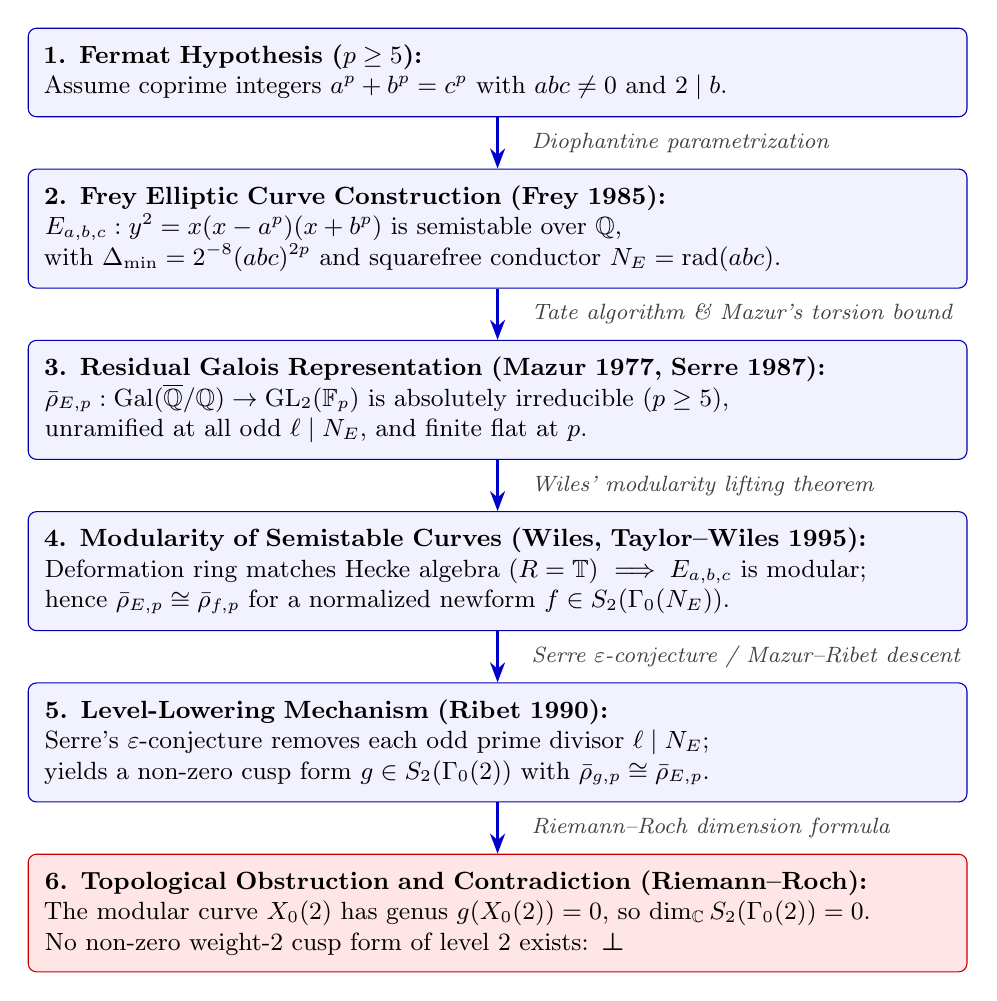
\begin{tikzpicture}[
    box/.style={rectangle, draw=blue!70!black, fill=blue!5, rounded corners=3pt, text width=11.5cm, minimum height=0.95cm, inner sep=6pt, font=\small},
    contra/.style={rectangle, draw=red!80!black, fill=red!10, rounded corners=3pt, text width=11.5cm, minimum height=0.95cm, inner sep=6pt, font=\small},
    arrow/.style={-{Stealth[scale=1.1]}, thick, draw=blue!80!black},
    annot/.style={font=\footnotesize\itshape, text=black!75, midway, right=0.3cm}
]

\node[box] (step1) {
    \textbf{1. Fermat Hypothesis ($p \ge 5$):}\\
    Assume coprime integers $a^p + b^p = c^p$ with $abc \neq 0$ and $2 \mid b$.
};

\node[box, below=0.65cm of step1] (step2) {
    \textbf{2. Frey Elliptic Curve Construction (Frey 1985):}\\
    $E_{a,b,c}: y^2 = x(x - a^p)(x + b^p)$ is semistable over $\Q$,\\
    with $\Delta_{\min} = 2^{-8}(abc)^{2p}$ and squarefree conductor $N_E = \mathrm{rad}(abc)$.
};

\node[box, below=0.65cm of step2] (step3) {
    \textbf{3. Residual Galois Representation (Mazur 1977, Serre 1987):}\\
    $\bar{\rho}_{E,p}: \Gal(\overline{\Q}/\Q) \to \GL_2(\F_p)$ is absolutely irreducible ($p \ge 5$),\\
    unramified at all odd $\ell \mid N_E$, and finite flat at $p$.
};

\node[box, below=0.65cm of step3] (step4) {
    \textbf{4. Modularity of Semistable Curves (Wiles, Taylor--Wiles 1995):}\\
    Deformation ring matches Hecke algebra ($R = \mathbb{T}$) $\implies E_{a,b,c}$ is modular;\\
    hence $\bar{\rho}_{E,p} \cong \bar{\rho}_{f,p}$ for a normalized newform $f \in S_2(\Gamma_0(N_E))$.
};

\node[box, below=0.65cm of step4] (step5) {
    \textbf{5. Level-Lowering Mechanism (Ribet 1990):}\\
    Serre's $\varepsilon$-conjecture removes each odd prime divisor $\ell \mid N_E$;\\
    yields a non-zero cusp form $g \in S_2(\Gamma_0(2))$ with $\bar{\rho}_{g,p} \cong \bar{\rho}_{E,p}$.
};

\node[contra, below=0.65cm of step5] (step6) {
    \textbf{6. Topological Obstruction and Contradiction (Riemann--Roch):}\\
    The modular curve $X_0(2)$ has genus $g(X_0(2)) = 0$, so $\dim_\C S_2(\Gamma_0(2)) = 0$.\\
    No non-zero weight-$2$ cusp form of level $2$ exists: $\boldsymbol{\bot}$
};

\draw[arrow] (step1) -- node[annot] {Diophantine parametrization} (step2);
\draw[arrow] (step2) -- node[annot] {Tate algorithm \& Mazur's torsion bound} (step3);
\draw[arrow] (step3) -- node[annot] {Wiles' modularity lifting theorem} (step4);
\draw[arrow] (step4) -- node[annot] {Serre $\varepsilon$-conjecture / Mazur--Ribet descent} (step5);
\draw[arrow] (step5) -- node[annot] {Riemann--Roch dimension formula} (step6);

\end{tikzpicture}
\caption{The deductive implication chain connecting Fermat's equation to the dimensional contradiction.}
\label{fig:logical-chain}
\end{figure}

\subsection{Synoptic Dependency Table}

Table~\ref{tab:logical-chain} summarizes each link in the logical chain, highlighting the formal theorem invoked and its decisive output.

\begin{table}[H]
\centering
\small
\begin{tabularx}{\textwidth}{l p{3.2cm} p{3.8cm} X}
\toprule
\textbf{Step} & \textbf{Input State} & \textbf{Governing Theorem} & \textbf{Decisive Consequence} \\
\midrule
1. Hypothesis & $a^p + b^p = c^p$, $p \ge 5$ & Diophantine reduction & Normalized solution with $2 \mid b$, $a \equiv -1 \pmod 4$ \\
2. Geometry & Frey curve $E_{a,b,c}$ & Tate algorithm~\cite{silverman2009} & Semistable curve; $\Delta_{\min} = 2^{-8}(abc)^{2p}$, $N_E = \mathrm{rad}(abc)$ \\
3. Galois Rep. & $E[p]$ torsion module & Mazur's Theorem~\cite{mazur1977} & $\bar{\rho}_{E,p}$ irreducible; unramified for odd $\ell \neq p$, flat at $p$ \\
4. Modularity & Semistable $E_{a,b,c}$ & Wiles--Taylor $R = \mathbb{T}$~\cite{wiles1995, taylorwiles1995} & $E$ is modular: $\bar{\rho}_{E,p} \cong \bar{\rho}_{f,p}$ for $f \in S_2(\Gamma_0(N_E))$ \\
5. Level-Lowering & Ramification at $\ell \mid N_E$ & Ribet's Theorem~\cite{ribet1990, serre1987} & Strips odd primes; descends to $g \in S_2(\Gamma_0(2))$ \\
6. Contradiction & Cusp form space $S_2(\Gamma_0(2))$ & Riemann--Roch~\cite{diamondshurman2005} & $\dim_\C S_2(\Gamma_0(2)) = g(X_0(2)) = 0 \implies \boldsymbol{\bot}$ \\
\bottomrule
\end{tabularx}
\caption{Systematic breakdown of the components connecting the Frey curve to the dimensional contradiction.}
\label{tab:logical-chain}
\end{table}

\subsection{The Five Foundational Pillars}

The logical rigidity of the proof rests on five interlocking theorems, each closing off any possible mathematical escape:
\begin{enumerate}
    \item \textbf{Hellegouarch--Frey Parity Normalization:} By requiring $2 \mid b$ and $a \equiv -1 \pmod 4$, the Frey curve exhibits multiplicative (rather than additive) reduction at $2$. This ensures semistability at \emph{all} primes, bounding the conductor at $2$ rather than higher powers of $2$.
    \item \textbf{Mazur's Torsion Bound:} A reducible $\bar{\rho}_{E,p}$ would imply the existence of a rational $p$-isogeny or rational $p$-torsion point on $E$. Mazur's theorem $X_0(p)(\Q) = \text{cusps}$ for $p > 13$ (and explicit checks for $p = 5, 7, 11, 13$) eliminates reducible representations for all primes $p \ge 5$.
    \item \textbf{Wiles' Modularity Lifting:} Wiles and Taylor established that the universal deformation ring $R$ is isomorphic to the Hecke algebra $\mathbb{T}$ for semistable elliptic curves, avoiding the general modularity conjecture while completely covering all Frey curves.
    \item \textbf{Serre's Conductor Formula and Ribet's Descent:} The conductor $N(\bar{\rho}_{E,p})$ of the residual representation excludes all odd prime factors because the valuation $v_\ell(\Delta_E) = 2p \cdot v_\ell(abc)$ is divisible by $p$. Ribet's theorem proves that the minimal modular level matches this Artin conductor outside $p$, leaving only the factor $2$.
    \item \textbf{Riemann--Roch on $X_0(2)$:} The modular curve $X_0(2) \cong \mathbb{P}^1_\C$ has genus $g = 0$. The space of holomorphic differentials $\Omega^1(X_0(2)) \cong S_2(\Gamma_0(2))$ is trivial, providing the definitive arithmetic-geometric barrier.
\end{enumerate}

\section{Conclusion}

The modern proof of Fermat's Last Theorem stands as one of the triumphant achievements of twentieth-century thought. By realizing Fermat's arithmetic assertion as an obstruction in the geometry of modular curves, the proof validated the profound Langlands philosophy that arithmetic representations and automorphic forms are reflections of the same underlying reality. Furthermore, its formal verification in Lean~4~\cite{anthropic2026} provides algorithmic certainty of its foundational completeness.

\begin{thebibliography}{99}

\bibitem{wiles1995}
Andrew Wiles.
\newblock Modular elliptic curves and Fermat's Last Theorem.
\newblock {\em Annals of Mathematics}, 141(3):443--551, 1995.

\bibitem{taylorwiles1995}
Richard Taylor and Andrew Wiles.
\newblock Ring-theoretic properties of certain Hecke algebras.
\newblock {\em Annals of Mathematics}, 141(3):553--572, 1995.

\bibitem{ribet1990}
Kenneth~A. Ribet.
\newblock On modular representations of $\mathrm{Gal}(\overline{\mathbb{Q}}/\mathbb{Q})$ arising from modular forms.
\newblock {\em Inventiones Mathematicae}, 100(1):431--476, 1990.

\bibitem{frey1986}
Gerhard Frey.
\newblock Links between stable elliptic curves and certain Diophantine equations.
\newblock {\em Annales Universitatis Saraviensis. Series Mathematicae}, 1(1):1--40, 1986.

\bibitem{serre1987}
Jean-Pierre Serre.
\newblock Sur les repr\'esentations modulaires de degr\'e 2 de $\mathrm{Gal}(\overline{\mathbb{Q}}/\mathbb{Q})$.
\newblock {\em Duke Mathematical Journal}, 54(1):179--230, 1987.

\bibitem{mazur1977}
Barry Mazur.
\newblock Modular curves and the Eisenstein ideal.
\newblock {\em Publications Math\'ematiques de l'IH\'ES}, 47:33--186, 1977.

\bibitem{ddt1997}
Henri Darmon, Fred Diamond, and Richard Taylor.
\newblock Fermat's Last Theorem.
\newblock In {\em Elliptic Curves, Modular Forms and Fermat's Last Theorem}, pages 2--140. International Press, Cambridge, MA, 1997.

\bibitem{silverman2009}
Joseph~H. Silverman.
\newblock {\em The Arithmetic of Elliptic Curves}, volume 106 of {\em Graduate Texts in Mathematics}.
\newblock Springer, New York, 2nd edition, 2009.

\bibitem{diamondshurman2005}
Fred Diamond and Jerry Shurman.
\newblock {\em A First Course in Modular Forms}, volume 228 of {\em Graduate Texts in Mathematics}.
\newblock Springer, New York, 2005.

\bibitem{anthropic2026}
Tianyi Peng et~al. (Anthropic).
\newblock Formalizing Fermat's Last Theorem.
\newblock {\em Anthropic Research}, September 4, 2026.
\newblock \url{https://www.anthropic.com/research/formalizing-fermats-last-theorem}.

\bibitem{prove2me2026}
Shuze Chen, Kunal Marwaha, Xiaoyang Lu, Henry Yuen, and Tianyi Peng.
\newblock Prove2Me: An open collaborative platform for scaling math formalization.
\newblock {\em arXiv preprint arXiv:2608.28433}, 2026.

\end{thebibliography}

\end{document}
